% Short Sectioned Assignment
% LaTeX Template
% Version 1.0 (5/5/12)
%
% This template has been downloaded from:
% http://www.LaTeXTemplates.com
%
% Original author:
% Frits Wenneker (http://www.howtotex.com)
%
% License:
% CC BY-NC-SA 3.0 (http://creativecommons.org/licenses/by-nc-sa/3.0/)
%
%%%%%%%%%%%%%%%%%%%%%%%%%%%%%%%%%%%%%%%%%

%----------------------------------------------------------------------------------------
%   PACKAGES AND OTHER DOCUMENT CONFIGURATIONS
%----------------------------------------------------------------------------------------

\documentclass[paper=a4, fontsize=11pt]{scrartcl} % A4 paper and 11pt font size

\usepackage[utf8]{inputenc}
\usepackage[T1]{fontenc} % Use 8-bit encoding that has 256 glyphs
\usepackage{fourier} % Use the Adobe Utopia font for the document - comment this line to return to the LaTeX default
\usepackage[norsk]{babel} % English language/hyphenation
\usepackage{amsmath,amsfonts,amsthm} % Math packages

\usepackage{lipsum} % Used for inserting dummy 'Lorem ipsum' text into the template
\usepackage{graphicx} % Used for graphs and images

\usepackage{sectsty} % Allows customizing section commands
\allsectionsfont{\centering \normalfont\scshape} % Make all sections centered, the default font and small caps

\usepackage{fancyhdr} % Custom headers and footers
\pagestyle{fancyplain} % Makes all pages in the document conform to the custom headers and footers
\fancyhead{} % No page header - if you want one, create it in the same way as the footers below
\fancyfoot[L]{} % Empty left footer
\fancyfoot[C]{} % Empty center footer
\fancyfoot[R]{\thepage} % Page numbering for right footer
\renewcommand{\headrulewidth}{0pt} % Remove header underlines
\renewcommand{\footrulewidth}{0pt} % Remove footer underlines
\setlength{\headheight}{13.6pt} % Customize the height of the header

\numberwithin{equation}{section} % Number equations within sections (i.e. 1.1, 1.2, 2.1, 2.2 instead of 1, 2, 3, 4)
\numberwithin{figure}{section} % Number figures within sections (i.e. 1.1, 1.2, 2.1, 2.2 instead of 1, 2, 3, 4)
\numberwithin{table}{section} % Number tables within sections (i.e. 1.1, 1.2, 2.1, 2.2 instead of 1, 2, 3, 4)

\setlength\parindent{0pt} % Removes all indentation from paragraphs - comment this line for an assignment with lots of text

%----------------------------------------------------------------------------------------
%   TITLE SECTION
%----------------------------------------------------------------------------------------

\newcommand{\horrule}[1]{\rule{\linewidth}{#1}} % Create horizontal rule command with 1 argument of height

\title{%
\normalfont \normalsize
\textsc{NTNU - MTDT - TDT4145} \\ [25pt] % Your university, school and/or department name(s)
\horrule{0.5pt} \\[0.4cm] % Thin top horizontal rule
\huge {Øving 1} \\ % The assignment title
\horrule{2pt} \\[0.5cm] % Thick bottom horizontal rule
}

\author{Øyvind Robertsen} % Your name

\date{\normalsize\today} % Today's date or a custom date

\begin{document}

\maketitle % Print the title

%----------------------------------------------------------------------------------------
%   PROBLEM 1
%----------------------------------------------------------------------------------------
\section*{Task 1}

\begin{figure}[h!]
\centering
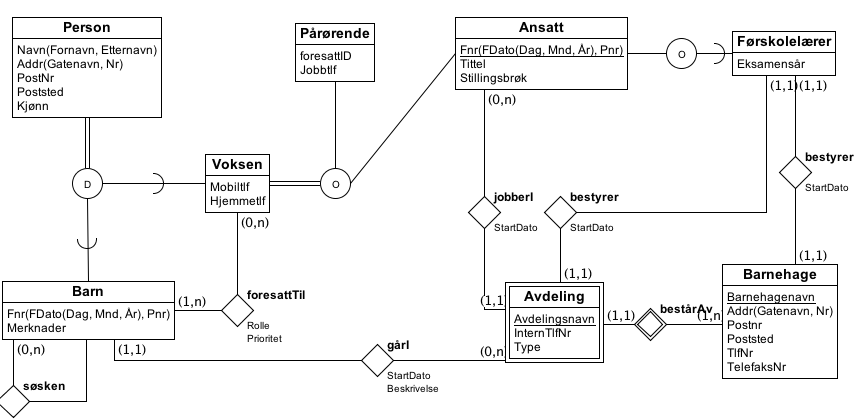
\includegraphics[width=\textwidth]{oppg1.png}
\caption{ER model for task 1}
\end{figure}

\newpage
%----------------------------------------------------------------------------------------
%   PROBLEM 1
%----------------------------------------------------------------------------------------
\section*{Task 2}

a)

\textbf{Person}(\underline{personnr}, navn, adresse, f.dato, kjønn, telefonnr, \underline{rådgiverPNr}, \underline{})

\textbf{Utdanning}(\underline{utdanningsId}, skole, antallÅr, grad, kursnavn)

\textbf{HarUtdanning}(\underline{personnr}, \underline{utdanningsID}, utdanningsÅr)

\textbf{Kompetanse}(\underline{kompetanseId}, område, stilling)

\textbf{HarKompetanse}(\underline{personnr}, \underline{kompetanseId}, grad)

\textbf{Oppdrag}(\underline{oppdragId}, \underline{utførtavPnr}, \underline{kundeNr}, stilling, fradato, tildato, lønn)

\textbf{Kunde}(\underline{kundeNr}, navn, adresse)

\vspace{1cm}

For å gjøre det enklere å refere mellom tabeller har jeg innført ekstra nøkkelatributter for noen av entitetene. Dette reduserer redundans.

Antar at rådgiverrelasjonen impliserer at vi ønsker å kunne finne en persons rådgiver ut fra en Person-instans, ikke alle person-instansene en person er rådgiver for.

\vspace{1cm}

b)

\begin{figure}[h!]
\centering
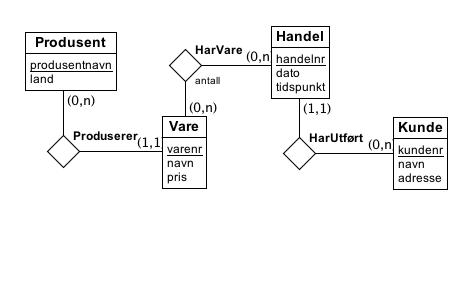
\includegraphics[width=\textwidth]{oppg2b.png}
\caption{ER model for task 2b}
\end{figure}

\end{document}

